% Created by tikzDevice version 0.8.1 on 2015-11-17 11:43:48
% !TEX encoding = UTF-8 Unicode
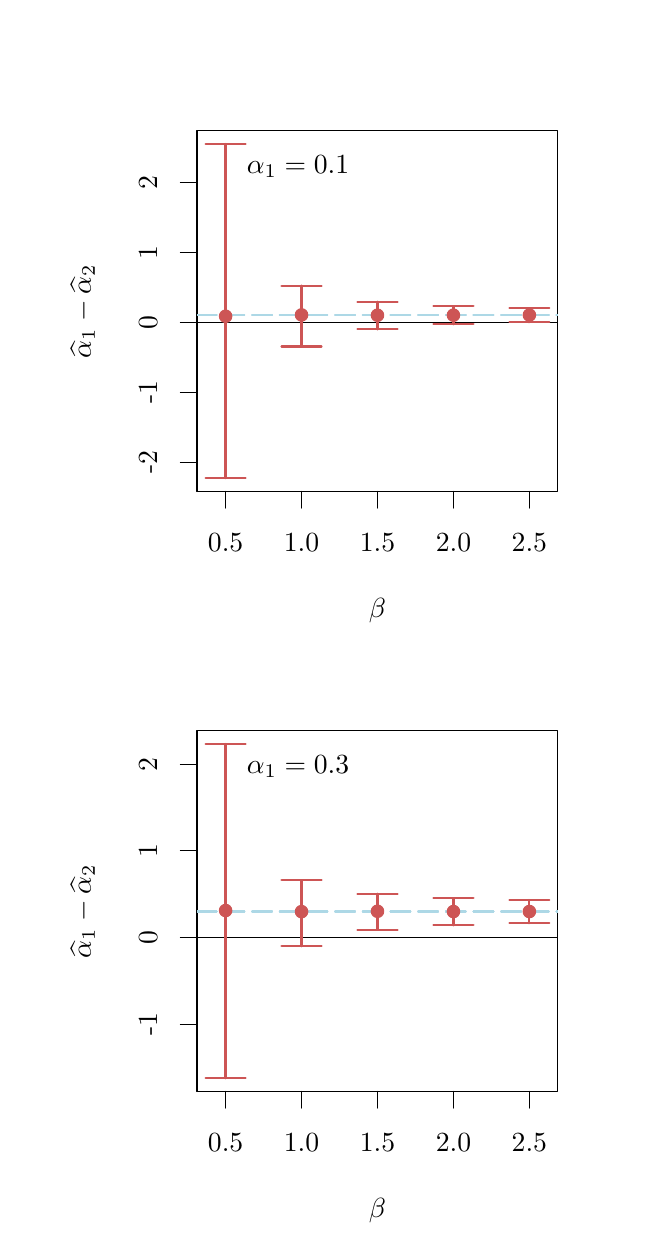
\begin{tikzpicture}[x=1pt,y=1pt]
\definecolor{fillColor}{RGB}{255,255,255}
\path[use as bounding box,fill=fillColor,fill opacity=0.00] (0,0) rectangle (216.81,433.62);
\begin{scope}
\path[clip] ( 61.20,266.01) rectangle (191.61,396.42);
\definecolor{drawColor}{RGB}{255,255,255}
\definecolor{fillColor}{RGB}{255,255,255}

\path[draw=drawColor,line width= 0.4pt,line join=round,line cap=round,fill=fillColor] ( 71.52,329.34) circle (  2.25);

\path[draw=drawColor,line width= 0.4pt,line join=round,line cap=round,fill=fillColor] ( 98.96,329.82) circle (  2.25);

\path[draw=drawColor,line width= 0.4pt,line join=round,line cap=round,fill=fillColor] (126.40,329.70) circle (  2.25);

\path[draw=drawColor,line width= 0.4pt,line join=round,line cap=round,fill=fillColor] (153.85,329.72) circle (  2.25);

\path[draw=drawColor,line width= 0.4pt,line join=round,line cap=round,fill=fillColor] (181.29,329.77) circle (  2.25);
\end{scope}
\begin{scope}
\path[clip] (  0.00,  0.00) rectangle (216.81,433.62);
\definecolor{drawColor}{RGB}{0,0,0}

\path[draw=drawColor,line width= 0.4pt,line join=round,line cap=round] ( 71.52,266.01) -- (181.29,266.01);

\path[draw=drawColor,line width= 0.4pt,line join=round,line cap=round] ( 71.52,266.01) -- ( 71.52,260.01);

\path[draw=drawColor,line width= 0.4pt,line join=round,line cap=round] ( 98.96,266.01) -- ( 98.96,260.01);

\path[draw=drawColor,line width= 0.4pt,line join=round,line cap=round] (126.40,266.01) -- (126.40,260.01);

\path[draw=drawColor,line width= 0.4pt,line join=round,line cap=round] (153.85,266.01) -- (153.85,260.01);

\path[draw=drawColor,line width= 0.4pt,line join=round,line cap=round] (181.29,266.01) -- (181.29,260.01);

\node[text=drawColor,anchor=base,inner sep=0pt, outer sep=0pt, scale=  1.00] at ( 71.52,244.41) {0.5};

\node[text=drawColor,anchor=base,inner sep=0pt, outer sep=0pt, scale=  1.00] at ( 98.96,244.41) {1.0};

\node[text=drawColor,anchor=base,inner sep=0pt, outer sep=0pt, scale=  1.00] at (126.40,244.41) {1.5};

\node[text=drawColor,anchor=base,inner sep=0pt, outer sep=0pt, scale=  1.00] at (153.85,244.41) {2.0};

\node[text=drawColor,anchor=base,inner sep=0pt, outer sep=0pt, scale=  1.00] at (181.29,244.41) {2.5};

\path[draw=drawColor,line width= 0.4pt,line join=round,line cap=round] ( 61.20,276.58) -- ( 61.20,377.74);

\path[draw=drawColor,line width= 0.4pt,line join=round,line cap=round] ( 61.20,276.58) -- ( 55.20,276.58);

\path[draw=drawColor,line width= 0.4pt,line join=round,line cap=round] ( 61.20,301.87) -- ( 55.20,301.87);

\path[draw=drawColor,line width= 0.4pt,line join=round,line cap=round] ( 61.20,327.16) -- ( 55.20,327.16);

\path[draw=drawColor,line width= 0.4pt,line join=round,line cap=round] ( 61.20,352.45) -- ( 55.20,352.45);

\path[draw=drawColor,line width= 0.4pt,line join=round,line cap=round] ( 61.20,377.74) -- ( 55.20,377.74);

\node[text=drawColor,rotate= 90.00,anchor=base,inner sep=0pt, outer sep=0pt, scale=  1.00] at ( 46.80,276.58) {-2};

\node[text=drawColor,rotate= 90.00,anchor=base,inner sep=0pt, outer sep=0pt, scale=  1.00] at ( 46.80,301.87) {-1};

\node[text=drawColor,rotate= 90.00,anchor=base,inner sep=0pt, outer sep=0pt, scale=  1.00] at ( 46.80,327.16) {0};

\node[text=drawColor,rotate= 90.00,anchor=base,inner sep=0pt, outer sep=0pt, scale=  1.00] at ( 46.80,352.45) {1};

\node[text=drawColor,rotate= 90.00,anchor=base,inner sep=0pt, outer sep=0pt, scale=  1.00] at ( 46.80,377.74) {2};

\path[draw=drawColor,line width= 0.4pt,line join=round,line cap=round] ( 61.20,266.01) --
	(191.61,266.01) --
	(191.61,396.42) --
	( 61.20,396.42) --
	( 61.20,266.01);
\end{scope}
\begin{scope}
\path[clip] (  0.00,216.81) rectangle (216.81,433.62);
\definecolor{drawColor}{RGB}{0,0,0}

\node[text=drawColor,anchor=base,inner sep=0pt, outer sep=0pt, scale=  1.00] at (126.41,220.41) {$\beta$};

\node[text=drawColor,rotate= 90.00,anchor=base,inner sep=0pt, outer sep=0pt, scale=  1.00] at ( 22.80,331.22) {$\widehat{\alpha}_1 - \widehat{\alpha}_2$};
\end{scope}
\begin{scope}
\path[clip] ( 61.20,266.01) rectangle (191.61,396.42);
\definecolor{drawColor}{RGB}{0,0,0}

\node[text=drawColor,anchor=base west,inner sep=0pt, outer sep=0pt, scale=  1.00] at ( 79.20,380.98) {$\alpha_1=0.1$};
\definecolor{drawColor}{RGB}{173,216,230}

\path[draw=drawColor,line width= 0.8pt,dash pattern=on 7pt off 3pt ,line join=round,line cap=round] ( 61.20,329.69) -- (191.61,329.69);

\path[draw=drawColor,line width= 0.8pt,dash pattern=on 7pt off 3pt ,line join=round,line cap=round] ( 61.20,329.69) -- (191.61,329.69);

\path[draw=drawColor,line width= 0.8pt,dash pattern=on 7pt off 3pt ,line join=round,line cap=round] ( 61.20,329.69) -- (191.61,329.69);

\path[draw=drawColor,line width= 0.8pt,dash pattern=on 7pt off 3pt ,line join=round,line cap=round] ( 61.20,329.69) -- (191.61,329.69);

\path[draw=drawColor,line width= 0.8pt,dash pattern=on 7pt off 3pt ,line join=round,line cap=round] ( 61.20,329.69) -- (191.61,329.69);
\definecolor{drawColor}{RGB}{0,0,0}

\path[draw=drawColor,line width= 0.4pt,line join=round,line cap=round] ( 61.20,327.16) -- (191.61,327.16);
\definecolor{drawColor}{RGB}{205,85,85}

\path[draw=drawColor,line width= 0.8pt,line join=round,line cap=round] ( 71.52,270.84) -- ( 71.52,391.59);

\path[draw=drawColor,line width= 0.8pt,line join=round,line cap=round] ( 64.29,270.84) --
	( 71.52,270.84) --
	( 78.75,270.84);

\path[draw=drawColor,line width= 0.8pt,line join=round,line cap=round] ( 78.75,391.59) --
	( 71.52,391.59) --
	( 64.29,391.59);

\path[draw=drawColor,line width= 0.8pt,line join=round,line cap=round] ( 98.96,318.37) -- ( 98.96,340.39);

\path[draw=drawColor,line width= 0.8pt,line join=round,line cap=round] ( 91.73,318.37) --
	( 98.96,318.37) --
	(106.19,318.37);

\path[draw=drawColor,line width= 0.8pt,line join=round,line cap=round] (106.19,340.39) --
	( 98.96,340.39) --
	( 91.73,340.39);

\path[draw=drawColor,line width= 0.8pt,line join=round,line cap=round] (126.40,324.60) -- (126.40,334.55);

\path[draw=drawColor,line width= 0.8pt,line join=round,line cap=round] (119.18,324.60) --
	(126.40,324.60) --
	(133.63,324.60);

\path[draw=drawColor,line width= 0.8pt,line join=round,line cap=round] (133.63,334.55) --
	(126.40,334.55) --
	(119.18,334.55);

\path[draw=drawColor,line width= 0.8pt,line join=round,line cap=round] (153.85,326.43) -- (153.85,332.91);

\path[draw=drawColor,line width= 0.8pt,line join=round,line cap=round] (146.62,326.43) --
	(153.85,326.43) --
	(161.08,326.43);

\path[draw=drawColor,line width= 0.8pt,line join=round,line cap=round] (161.08,332.91) --
	(153.85,332.91) --
	(146.62,332.91);

\path[draw=drawColor,line width= 0.8pt,line join=round,line cap=round] (181.29,327.16) -- (181.29,332.21);

\path[draw=drawColor,line width= 0.8pt,line join=round,line cap=round] (174.06,327.16) --
	(181.29,327.16) --
	(188.52,327.16);

\path[draw=drawColor,line width= 0.8pt,line join=round,line cap=round] (188.52,332.21) --
	(181.29,332.21) --
	(174.06,332.21);
\definecolor{fillColor}{RGB}{205,85,85}

\path[draw=drawColor,line width= 0.4pt,line join=round,line cap=round,fill=fillColor] ( 71.52,329.34) circle (  2.25);

\path[draw=drawColor,line width= 0.4pt,line join=round,line cap=round,fill=fillColor] ( 98.96,329.82) circle (  2.25);

\path[draw=drawColor,line width= 0.4pt,line join=round,line cap=round,fill=fillColor] (126.40,329.70) circle (  2.25);

\path[draw=drawColor,line width= 0.4pt,line join=round,line cap=round,fill=fillColor] (153.85,329.72) circle (  2.25);

\path[draw=drawColor,line width= 0.4pt,line join=round,line cap=round,fill=fillColor] (181.29,329.77) circle (  2.25);
\end{scope}
\begin{scope}
\path[clip] ( 61.20, 49.20) rectangle (191.61,179.61);
\definecolor{drawColor}{RGB}{255,255,255}
\definecolor{fillColor}{RGB}{255,255,255}

\path[draw=drawColor,line width= 0.4pt,line join=round,line cap=round,fill=fillColor] ( 71.52,114.59) circle (  2.25);

\path[draw=drawColor,line width= 0.4pt,line join=round,line cap=round,fill=fillColor] ( 98.96,114.20) circle (  2.25);

\path[draw=drawColor,line width= 0.4pt,line join=round,line cap=round,fill=fillColor] (126.40,114.33) circle (  2.25);

\path[draw=drawColor,line width= 0.4pt,line join=round,line cap=round,fill=fillColor] (153.85,114.23) circle (  2.25);

\path[draw=drawColor,line width= 0.4pt,line join=round,line cap=round,fill=fillColor] (181.29,114.24) circle (  2.25);
\end{scope}
\begin{scope}
\path[clip] (  0.00,  0.00) rectangle (216.81,433.62);
\definecolor{drawColor}{RGB}{0,0,0}

\path[draw=drawColor,line width= 0.4pt,line join=round,line cap=round] ( 71.52, 49.20) -- (181.29, 49.20);

\path[draw=drawColor,line width= 0.4pt,line join=round,line cap=round] ( 71.52, 49.20) -- ( 71.52, 43.20);

\path[draw=drawColor,line width= 0.4pt,line join=round,line cap=round] ( 98.96, 49.20) -- ( 98.96, 43.20);

\path[draw=drawColor,line width= 0.4pt,line join=round,line cap=round] (126.40, 49.20) -- (126.40, 43.20);

\path[draw=drawColor,line width= 0.4pt,line join=round,line cap=round] (153.85, 49.20) -- (153.85, 43.20);

\path[draw=drawColor,line width= 0.4pt,line join=round,line cap=round] (181.29, 49.20) -- (181.29, 43.20);

\node[text=drawColor,anchor=base,inner sep=0pt, outer sep=0pt, scale=  1.00] at ( 71.52, 27.60) {0.5};

\node[text=drawColor,anchor=base,inner sep=0pt, outer sep=0pt, scale=  1.00] at ( 98.96, 27.60) {1.0};

\node[text=drawColor,anchor=base,inner sep=0pt, outer sep=0pt, scale=  1.00] at (126.40, 27.60) {1.5};

\node[text=drawColor,anchor=base,inner sep=0pt, outer sep=0pt, scale=  1.00] at (153.85, 27.60) {2.0};

\node[text=drawColor,anchor=base,inner sep=0pt, outer sep=0pt, scale=  1.00] at (181.29, 27.60) {2.5};

\path[draw=drawColor,line width= 0.4pt,line join=round,line cap=round] ( 61.20, 73.53) -- ( 61.20,167.47);

\path[draw=drawColor,line width= 0.4pt,line join=round,line cap=round] ( 61.20, 73.53) -- ( 55.20, 73.53);

\path[draw=drawColor,line width= 0.4pt,line join=round,line cap=round] ( 61.20,104.85) -- ( 55.20,104.85);

\path[draw=drawColor,line width= 0.4pt,line join=round,line cap=round] ( 61.20,136.16) -- ( 55.20,136.16);

\path[draw=drawColor,line width= 0.4pt,line join=round,line cap=round] ( 61.20,167.47) -- ( 55.20,167.47);

\node[text=drawColor,rotate= 90.00,anchor=base,inner sep=0pt, outer sep=0pt, scale=  1.00] at ( 46.80, 73.53) {-1};

\node[text=drawColor,rotate= 90.00,anchor=base,inner sep=0pt, outer sep=0pt, scale=  1.00] at ( 46.80,104.85) {0};

\node[text=drawColor,rotate= 90.00,anchor=base,inner sep=0pt, outer sep=0pt, scale=  1.00] at ( 46.80,136.16) {1};

\node[text=drawColor,rotate= 90.00,anchor=base,inner sep=0pt, outer sep=0pt, scale=  1.00] at ( 46.80,167.47) {2};

\path[draw=drawColor,line width= 0.4pt,line join=round,line cap=round] ( 61.20, 49.20) --
	(191.61, 49.20) --
	(191.61,179.61) --
	( 61.20,179.61) --
	( 61.20, 49.20);
\end{scope}
\begin{scope}
\path[clip] (  0.00,  0.00) rectangle (216.81,216.81);
\definecolor{drawColor}{RGB}{0,0,0}

\node[text=drawColor,anchor=base,inner sep=0pt, outer sep=0pt, scale=  1.00] at (126.41,  3.60) {$\beta$};

\node[text=drawColor,rotate= 90.00,anchor=base,inner sep=0pt, outer sep=0pt, scale=  1.00] at ( 22.80,114.41) {$\widehat{\alpha}_1 - \widehat{\alpha}_2$};
\end{scope}
\begin{scope}
\path[clip] ( 61.20, 49.20) rectangle (191.61,179.61);
\definecolor{drawColor}{RGB}{0,0,0}

\node[text=drawColor,anchor=base west,inner sep=0pt, outer sep=0pt, scale=  1.00] at ( 79.20,164.17) {$\alpha_1=0.3$};
\definecolor{drawColor}{RGB}{173,216,230}

\path[draw=drawColor,line width= 0.8pt,dash pattern=on 7pt off 3pt ,line join=round,line cap=round] ( 61.20,114.24) -- (191.61,114.24);

\path[draw=drawColor,line width= 0.8pt,dash pattern=on 7pt off 3pt ,line join=round,line cap=round] ( 61.20,114.24) -- (191.61,114.24);

\path[draw=drawColor,line width= 0.8pt,dash pattern=on 7pt off 3pt ,line join=round,line cap=round] ( 61.20,114.24) -- (191.61,114.24);

\path[draw=drawColor,line width= 0.8pt,dash pattern=on 7pt off 3pt ,line join=round,line cap=round] ( 61.20,114.24) -- (191.61,114.24);

\path[draw=drawColor,line width= 0.8pt,dash pattern=on 7pt off 3pt ,line join=round,line cap=round] ( 61.20,114.24) -- (191.61,114.24);
\definecolor{drawColor}{RGB}{0,0,0}

\path[draw=drawColor,line width= 0.4pt,line join=round,line cap=round] ( 61.20,104.85) -- (191.61,104.85);
\definecolor{drawColor}{RGB}{205,85,85}

\path[draw=drawColor,line width= 0.8pt,line join=round,line cap=round] ( 71.52, 54.03) -- ( 71.52,174.78);

\path[draw=drawColor,line width= 0.8pt,line join=round,line cap=round] ( 64.29, 54.03) --
	( 71.52, 54.03) --
	( 78.75, 54.03);

\path[draw=drawColor,line width= 0.8pt,line join=round,line cap=round] ( 78.75,174.78) --
	( 71.52,174.78) --
	( 64.29,174.78);

\path[draw=drawColor,line width= 0.8pt,line join=round,line cap=round] ( 98.96,101.72) -- ( 98.96,125.52);

\path[draw=drawColor,line width= 0.8pt,line join=round,line cap=round] ( 91.73,101.72) --
	( 98.96,101.72) --
	(106.19,101.72);

\path[draw=drawColor,line width= 0.8pt,line join=round,line cap=round] (106.19,125.52) --
	( 98.96,125.52) --
	( 91.73,125.52);

\path[draw=drawColor,line width= 0.8pt,line join=round,line cap=round] (126.40,107.67) -- (126.40,120.66);

\path[draw=drawColor,line width= 0.8pt,line join=round,line cap=round] (119.18,107.67) --
	(126.40,107.67) --
	(133.63,107.67);

\path[draw=drawColor,line width= 0.8pt,line join=round,line cap=round] (133.63,120.66) --
	(126.40,120.66) --
	(119.18,120.66);

\path[draw=drawColor,line width= 0.8pt,line join=round,line cap=round] (153.85,109.25) -- (153.85,119.07);

\path[draw=drawColor,line width= 0.8pt,line join=round,line cap=round] (146.62,109.25) --
	(153.85,109.25) --
	(161.08,109.25);

\path[draw=drawColor,line width= 0.8pt,line join=round,line cap=round] (161.08,119.07) --
	(153.85,119.07) --
	(146.62,119.07);

\path[draw=drawColor,line width= 0.8pt,line join=round,line cap=round] (181.29,109.96) -- (181.29,118.37);

\path[draw=drawColor,line width= 0.8pt,line join=round,line cap=round] (174.06,109.96) --
	(181.29,109.96) --
	(188.52,109.96);

\path[draw=drawColor,line width= 0.8pt,line join=round,line cap=round] (188.52,118.37) --
	(181.29,118.37) --
	(174.06,118.37);
\definecolor{fillColor}{RGB}{205,85,85}

\path[draw=drawColor,line width= 0.4pt,line join=round,line cap=round,fill=fillColor] ( 71.52,114.59) circle (  2.25);

\path[draw=drawColor,line width= 0.4pt,line join=round,line cap=round,fill=fillColor] ( 98.96,114.20) circle (  2.25);

\path[draw=drawColor,line width= 0.4pt,line join=round,line cap=round,fill=fillColor] (126.40,114.33) circle (  2.25);

\path[draw=drawColor,line width= 0.4pt,line join=round,line cap=round,fill=fillColor] (153.85,114.23) circle (  2.25);

\path[draw=drawColor,line width= 0.4pt,line join=round,line cap=round,fill=fillColor] (181.29,114.24) circle (  2.25);
\end{scope}
\end{tikzpicture}
